% Provenance (never printed): old seconde/premiere S material on the water
% cycle on land (the drainage basin, river discharge, floods and their
% management); see sources/book2/PROVENANCE.md. The Varden basin is computed
% in figdata/grade-10/varden_basin.py from figdata/shared/region.py; the
% Potomac record in figdata/grade-10/flood_frequency.py.
\chapter{Daerah Aliran Sungai, Sungai, dan Banjir}\label{ch:g10:drainage-basins}

Sebuah sungai dapat naik dua hari setelah hujan berhenti, di sebuah kota yang
sama sekali tidak kehujanan. Air yang membanjiri jalan-jalannya jatuh lebih
awal, di perbukitan jauh di hulu; air itu mengalir menuruni lereng-lereng ke
dalam anak-anak sungai, dan anak-anak sungai itu bergabung menjadi sungai yang
membawanya, sekaligus, ke kota itu. Untuk memahami banjir, kita harus melihat
melampaui sungai itu, ke seluruh wilayah yang memasoknya, dan mengikuti air
melalui wilayah itu. Bab ini mendefinisikan wilayah itu, \omterm{def:g10:drainage-basins:drainage-basin}{daerah aliran sungai};
mengukur apa yang dibawa sungai, yaitu \omterm{def:g10:drainage-basins:discharge}{debitnya}; mengikuti banjir ketika
melewati suatu titik di sungai; dan memperlihatkan bagaimana catatan banjir
yang panjang memberi tahu seberapa sering banjir tertentu datang kembali.

\begin{omfigure}
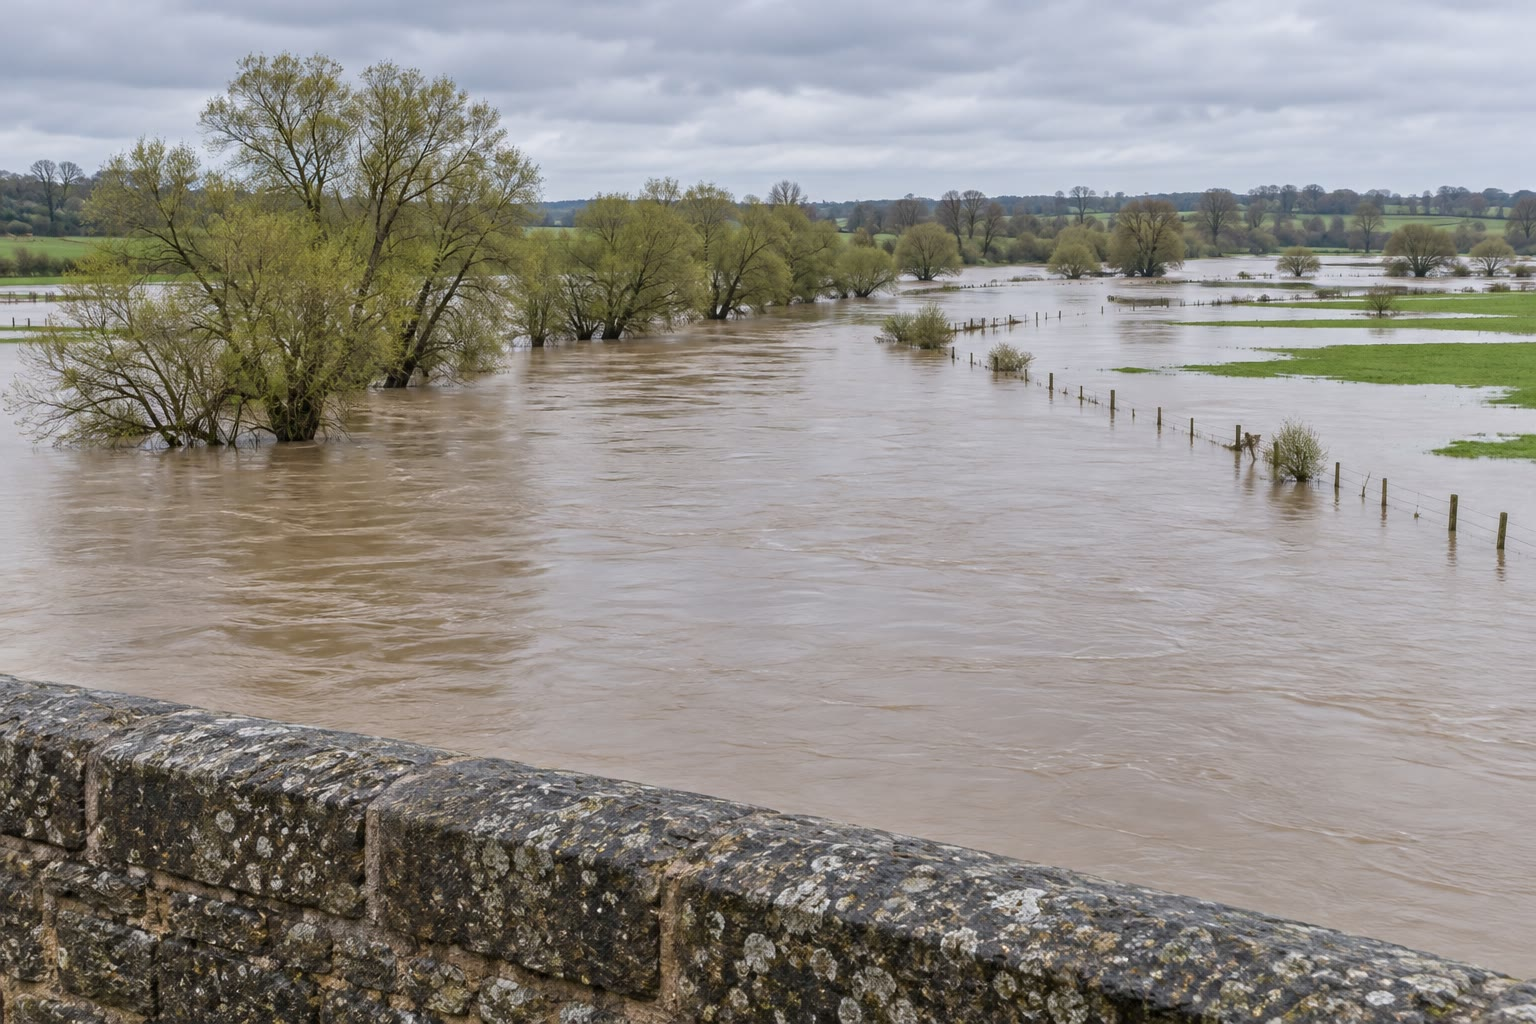
\includegraphics[width=0.8\linewidth]{images/book2/ai/g10-river-flood-meadows.jpg}

{\small Sungai yang sedang banjir, dilihat dari jembatan batu: air cokelat
yang sarat lumpur telah meninggalkan alurnya dan menutupi padang rumput di
dataran banjirnya, sampai ke pagar-pagar dan pohon-pohon yang berjajar di
tepiannya yang biasa.}
\end{omfigure}

\begin{recall}
Hujan yang mencapai tanah meresap ke dalamnya, mengalir di permukaannya, atau
menguap; daur air membawanya kembali ke laut (buku-buku fisika). Air meresap
ke dalam batuan yang permeabel dan mengisinya di bawah muka air tanah,
membentuk akuifer yang memasok mata air dan sungai (Buku 1, kelas 6). Sungai
berkelok-kelok membentuk meander di dataran banjirnya yang datar, yang
digenanginya ketika banjir (Buku 1, kelas 5). Garis kontur menghubungkan
titik-titik yang ketinggiannya sama; Perbukitan Varden adalah wilayah yang
digambar pada peta-peta seri ini (Buku 1, kelas 2 dan 9).
\end{recall}

\begin{safety}
Air banjir jauh lebih berbahaya daripada kelihatannya. Air yang mengalir deras
setinggi sekitar \qty{15}{cm} dapat menjatuhkan orang dewasa, dan setinggi
sekitar \qty{30}{cm} dapat menghanyutkan mobil; jalan di bawahnya mungkin
telah runtuh. Jangan pernah berjalan atau berkendara memasuki air banjir:
berbaliklah dan carilah jalan lain.
% ledger: nws:flood-water
\end{safety}

\section{Daerah aliran sungai}

Setiap tetes hujan yang tidak menguap atau meresap dalam-dalam mengalir
menuruni lereng. Tetes itu mengikuti kemiringan tanah yang paling curam,
bergabung dengan alur kecil, lalu dengan anak sungai, dan anak-anak sungai
bergabung menjadi sungai. Seluruh daratan yang airnya berakhir di sungai yang
sama membentuk satu kesatuan.

\begin{definition}[Daerah aliran sungai; garis pemisah air]\label{def:g10:drainage-basins:drainage-basin}
Yang disebut \emph{daerah aliran sungai}\index{daerah aliran sungai} untuk
suatu titik di sungai adalah seluruh wilayah daratan yang air lariannya
mengalir ke sungai di hulu titik itu dan melewati titik itu. Yang disebut
\emph{garis pemisah air}\index{garis pemisah air} adalah garis yang memisahkan
dua daerah aliran sungai yang bertetangga: garis itu mengikuti punggung-punggung
daratan, dan hujan yang jatuh di kedua sisinya mengalir ke sungai yang
berbeda.
\end{definition}

\omterm{def:g10:drainage-basins:drainage-basin}{Daerah aliran sungai} selalu didefinisikan untuk suatu titik di sungai, yaitu
\emph{titik keluarannya}: \omterm{def:g10:drainage-basins:drainage-basin}{daerah aliran sungai} di tempat sungai mencapai laut
adalah yang terluas, dan setiap titik di hulunya memiliki daerah aliran yang
lebih kecil di dalamnya. Dua tetes yang jatuh berjarak satu meter, di kedua
sisi \omterm{def:g10:drainage-basins:drainage-basin}{garis pemisah air}, dapat berakhir di sungai yang berbeda dan bahkan di
samudra yang berbeda.

\subsection*{Daerah aliran Sungai Varden}

Komputer menemukan \omterm{def:g10:drainage-basins:drainage-basin}{daerah aliran sungai} dari peta ketinggian dalam beberapa
langkah. Peta itu dipotong menjadi persegi-persegi kecil, di sini bersisi
\qty{50}{m}. Untuk setiap persegi, komputer memeriksa delapan tetangganya dan
mengirim air ke tetangga yang dicapai melalui kemiringan turun yang paling
curam. (Di tempat cekungan kecil tidak memiliki tetangga yang lebih rendah,
cekungan itu terlebih dahulu diisi sampai aras tempat airnya akan meluap,
seperti genangan.) Dengan mengikuti langkah-langkah ini dari persegi ke
persegi, kita dapat melacak jalan sebuah tetes dari mana pun di peta.
Persegi-persegi yang tetesnya mencapai sungai membentuk \omterm{def:g10:drainage-basins:drainage-basin}{daerah aliran sungai}
itu.

\begin{omfigure}
\begin{tikzpicture}
\begin{axis}[axis equal image, xmin=0, xmax=10, ymin=0, ymax=8, width=0.86\linewidth,
  tick label style={font=\scriptsize}, xlabel={timur (km)}, ylabel={utara (km)},
  label style={font=\small}, enlargelimits=false]
\addplot[fill=omDef!14, draw=none, even odd rule] table {figdata/out/grade-10-varden_basin-fill.dat};
\addplot[contour, line width=0.25pt, opacity=0.7] table {figdata/out/shared-region-contours.dat};
\addplot[index contour, opacity=0.8] table {figdata/out/shared-region-index-contours.dat};
\addplot[river, line width=1.6pt] table {figdata/out/shared-region-river.dat};
\addplot[omThm, line width=1.4pt, dashed] table {figdata/out/grade-10-varden_basin-divide.dat};
\addplot[omWxRain, line width=0.9pt, -{Stealth[length=5pt]}] table {figdata/out/grade-10-varden_basin-path1.dat};
\addplot[omWxRain, line width=0.9pt, -{Stealth[length=5pt]}] table {figdata/out/grade-10-varden_basin-path2.dat};
\addplot[omWxRain, line width=0.9pt, -{Stealth[length=5pt]}] table {figdata/out/grade-10-varden_basin-path3.dat};
\addplot[omWxRain, line width=0.9pt, -{Stealth[length=5pt]}] table {figdata/out/grade-10-varden_basin-path4.dat};
\fill[omWxRain] (axis cs:2,7.4) circle (2.2pt);
\fill[omWxRain] (axis cs:4,1.8) circle (2.2pt);
\fill[omWxRain] (axis cs:8.6,6.6) circle (2.2pt);
\fill[omWxRain] (axis cs:2.5,0.7) circle (2.2pt);
\node[font=\footnotesize, fill=white, fill opacity=0.85, text opacity=1, inner sep=1.5pt, text=omThm] at (axis cs:6.0,6.75) {pemisah air};
\node[font=\footnotesize, fill=white, fill opacity=0.85, text opacity=1, inner sep=1.5pt, text=omThm] at (axis cs:3.5,1.1) {pemisah air};
\node[font=\footnotesize, fill=white, fill opacity=0.85, text opacity=1, inner sep=1.5pt, align=center] at (axis cs:5.3,7.55) {di luar daerah aliran:\\air keluar ke utara};
\node[font=\footnotesize, fill=white, fill opacity=0.85, text opacity=1, inner sep=1.5pt, align=right, anchor=east] at (axis cs:9.85,3.35) {titik keluaran};
\draw[-{Stealth[length=6pt]}, line width=1pt, omRiver] (axis cs:9.3,3.7) -- (axis cs:9.95,4.15);
\node[font=\footnotesize, fill=white, fill opacity=0.85, text opacity=1, inner sep=1.5pt] at (axis cs:1.1,4.75) {sungai};
\end{axis}
\end{tikzpicture}

{\small Daerah aliran Sungai Varden pada peta Perbukitan Varden (diarsir),
dihitung dengan mengirim air dari setiap persegi \qty{50}{m} menuruni
kemiringan yang paling curam; kontur setiap \qty{50}{m}. Garis-garis
putus-putus adalah \omterm{def:g10:drainage-basins:drainage-basin}{garis pemisah air}; garis-garis biru adalah jalan empat
tetes hujan (titik). Dua tetes mencapai sungai dan mengalir ke timur menuju
titik keluaran, tempat sungai meninggalkan peta; dua tetes lainnya, di luar
\omterm{def:g10:drainage-basins:drainage-basin}{garis pemisah air}, meninggalkan peta menuju sungai-sungai lain.}
\end{omfigure}

Daerah aliran itu meliputi \qty{66}{km^2} dari \qty{80}{km^2} luas peta,
sekitar empat per lima bagiannya. Di utara, \omterm{def:g10:drainage-basins:drainage-basin}{garis pemisah air} mengikuti
punggung perbukitan dan melewati puncak-puncaknya; di baliknya daratan miring
menjauhi sungai dan airnya mengalir ke lembah lain. Di sudut barat daya,
sebuah wilayah kecil juga mengalirkan airnya ke luar peta. Sungai itu sendiri
memasuki peta dari barat, sehingga daerah alirannya yang lengkap lebih luas:
daerah aliran itu juga mencakup daratan di hulu, di luar tepi peta.
% values computed in figdata/grade-10/varden_basin.py (basin_km2 66.19, map_km2 80)

\subsection*{Sungai-sungai terbesar}

Sungai-sungai dibandingkan menurut luas daerah alirannya dan menurut air yang
dibawanya. Sungai terbesar di dunia, dengan selisih yang jauh, adalah Amazon.
Mississippi, sungai terbesar di Amerika Serikat, mengeringkan sekitar
\num{1150000} mil persegi, sekitar 2.98 juta \unit{km^2}, dari Amerika Serikat
dan Kanada.
% ledger: kammerer:mississippi

\section{Debit}

\begin{definition}[Debit]\label{def:g10:drainage-basins:discharge}
Yang disebut \emph{debit}\index{debit} sungai di suatu titik adalah volume air
yang melewati sebuah penampang sungai dalam satu detik. Debit diukur dalam
meter kubik per detik, \unit{m^3/s}.
\end{definition}

\omterm{def:g10:drainage-basins:discharge}{Debit} \qty{1}{m^3/s} adalah seribu liter setiap detik, atau
\qty{86400}{m^3} sehari. Air mengalir paling cepat di dekat permukaan di
tengah alur dan paling lambat di sepanjang dasar dan tepiannya, tempat air
bergesekan dengannya; \emph{kecepatan rata-rata} adalah kecepatan yang
dirata-ratakan atas seluruh penampang.

\begin{proposition}[Debit, kecepatan, dan penampang]\label{prop:g10:drainage-basins:discharge}
\omterm{def:g10:drainage-basins:discharge}{Debit} $Q$ sungai adalah hasil kali kecepatan rata-rata $v$ air dan luas $A$
penampang basah:
\[
Q = v\,A.
\]
\end{proposition}

\begin{proof}
Dalam waktu $t$, air yang melintasi penampang itu telah bergerak maju sejauh
$v\,t$: air itu mengisi sepotong sungai dengan penampang $A$ dan panjang
$v\,t$, yang volumenya $A\,v\,t$. Membagi volume ini dengan waktu $t$
memberikan volume per detik, $Q = v\,A$.
\end{proof}

Sungai dengan penampang \qty{50}{m^2} yang mengalir dengan kecepatan rata-rata
\qty{1.2}{m/s} membawa $1.2 \times 50 = \qty{60}{m^3/s}$. Saat banjir, kedua
faktor itu bertambah: air menjadi lebih dalam dan lebih lebar, sehingga
penampangnya bertambah, dan air mengalir lebih cepat.

\subsection*{Mengukur debit}

Karena kecepatan berubah dari tepi ke tepi sungai, kecepatan itu diukur di
beberapa titik. Sungai dipotong menjadi pita-pita tegak; di setiap pita,
kedalaman dan kecepatan diukur, dan \omterm{def:g10:drainage-basins:discharge}{debit} pita-pita itu dijumlahkan.

\begin{method}[Metode kecepatan--luas]\label{met:g10:drainage-basins:velocity-area}
\begin{enumerate}
  \item Bentangkan pita ukur melintasi sungai dan pilih garis-garis tegak
        dengan jarak teratur $w$ di sepanjangnya.
  \item Di setiap garis tegak, ukur kedalaman $d$ dan kecepatan rata-rata $v$
        air sepanjang kedalaman itu dengan pengukur arus.
  \item Setiap garis tegak mewakili sebuah pita selebar $w$ dengan luas
        $w\,d$; \omterm{def:g10:drainage-basins:discharge}{debitnya} $v\,w\,d$.
  \item Jumlahkan \omterm{def:g10:drainage-basins:discharge}{debit} semua pita: $Q = \sum v\,w\,d$.
        Penampangnya $A = \sum w\,d$ dan kecepatan rata-ratanya $Q/A$.
\end{enumerate}
\end{method}

\begin{omfigure}
\begin{tikzpicture}[x=0.9cm, y=1.6cm, font=\footnotesize]
  % water
  \fill[omSea] (0,0) -- (1,-0.4) -- (2,-0.75) -- (3,-1.0) -- (4,-1.25) -- (5,-1.4) -- (6,-1.3)
     -- (7,-1.1) -- (8,-0.8) -- (9,-0.5) -- (10,-0.2) -- (10.5,0) -- cycle;
  \fill[omDef!22] (4,0) -- (4,-1.25) -- (5,-1.4) -- (6,-1.3) -- (6,0) -- cycle;
  % bed
  \draw[line width=0.9pt, brown!60!black] (-0.6,0.35) -- (0,0) -- (1,-0.4) -- (2,-0.75) -- (3,-1.0) -- (4,-1.25)
     -- (5,-1.4) -- (6,-1.3) -- (7,-1.1) -- (8,-0.8) -- (9,-0.5) -- (10,-0.2) -- (10.5,0) -- (11.1,0.35);
  \draw[omDef!70!black, line width=0.5pt] (0,0) -- (10.5,0);
  % verticals
  \foreach \x/\d/\v/\dx in {1/0.4/0.3/0.3, 3/1.0/0.6/0, 5/1.4/0.8/0, 7/1.1/0.7/0, 9/0.5/0.4/-0.25} {
    \draw[black!70, dashed] (\x,0) -- (\x,-\d);
    \node[anchor=south, font=\scriptsize] at (\x,0.02) {\qty{\v}{m/s}};
    \node[font=\scriptsize, fill=white, inner sep=0.8pt] at (\x+\dx,-0.5*\d) {\qty{\d}{m}};
  }
  \draw[{Stealth}-{Stealth}] (4,0.42) -- node[above, font=\scriptsize] {satu pita: $w = \qty{2}{m}$} (6,0.42);
  \node[anchor=west, align=left] at (11.2,-0.15) {permukaan\\air};
  \node[anchor=west, align=left] at (11.2,-0.9) {dasar};
  \draw[black!50] (11.15,-0.9) -- (8.5,-0.68);
  \node[anchor=north] at (5.25,-1.75) {kecepatan rata-rata yang diukur di garis-garis tegak (di atas air) dan kedalaman (di dalam air)};
\end{tikzpicture}

{\small Mengukur \omterm{def:g10:drainage-basins:discharge}{debit} (skematis; skala tegak dibesar-besarkan). Lima garis
tegak, berjarak \qty{2}{m}, membagi sebuah anak sungai selebar sekitar
\qty{10}{m} menjadi pita-pita; pita yang diarsir adalah pita yang diukur di
garis tegak tengah.}
\end{omfigure}

\begin{example}[Sebuah pengukuran debit]\label{ex:g10:drainage-basins:gauging}
Pada anak sungai dalam gambar, kelima pita, yang masing-masing selebar
\qty{2}{m}, memiliki luas $2 \times 0.4 = 0.8$, $2.0$, $2.8$, $2.2$, dan
\qty{1.0}{m^2}: penampangnya \qty{8.8}{m^2}. \omterm{def:g10:drainage-basins:discharge}{Debitnya} $0.3 \times 0.8 =
0.24$, $0.6 \times 2.0 = 1.20$, $0.8 \times 2.8 = 2.24$, $0.7 \times 2.2 =
1.54$, dan $0.4 \times 1.0 = \qty{0.40}{m^3/s}$, sehingga anak sungai itu
membawa $Q \approx \qty{5.6}{m^3/s}$. Kecepatan rata-ratanya $5.62/8.8 \approx
\qty{0.64}{m/s}$, kurang dari \qty{0.8}{m/s} di bagian tengah aliran.
\end{example}

\begin{omfigure}
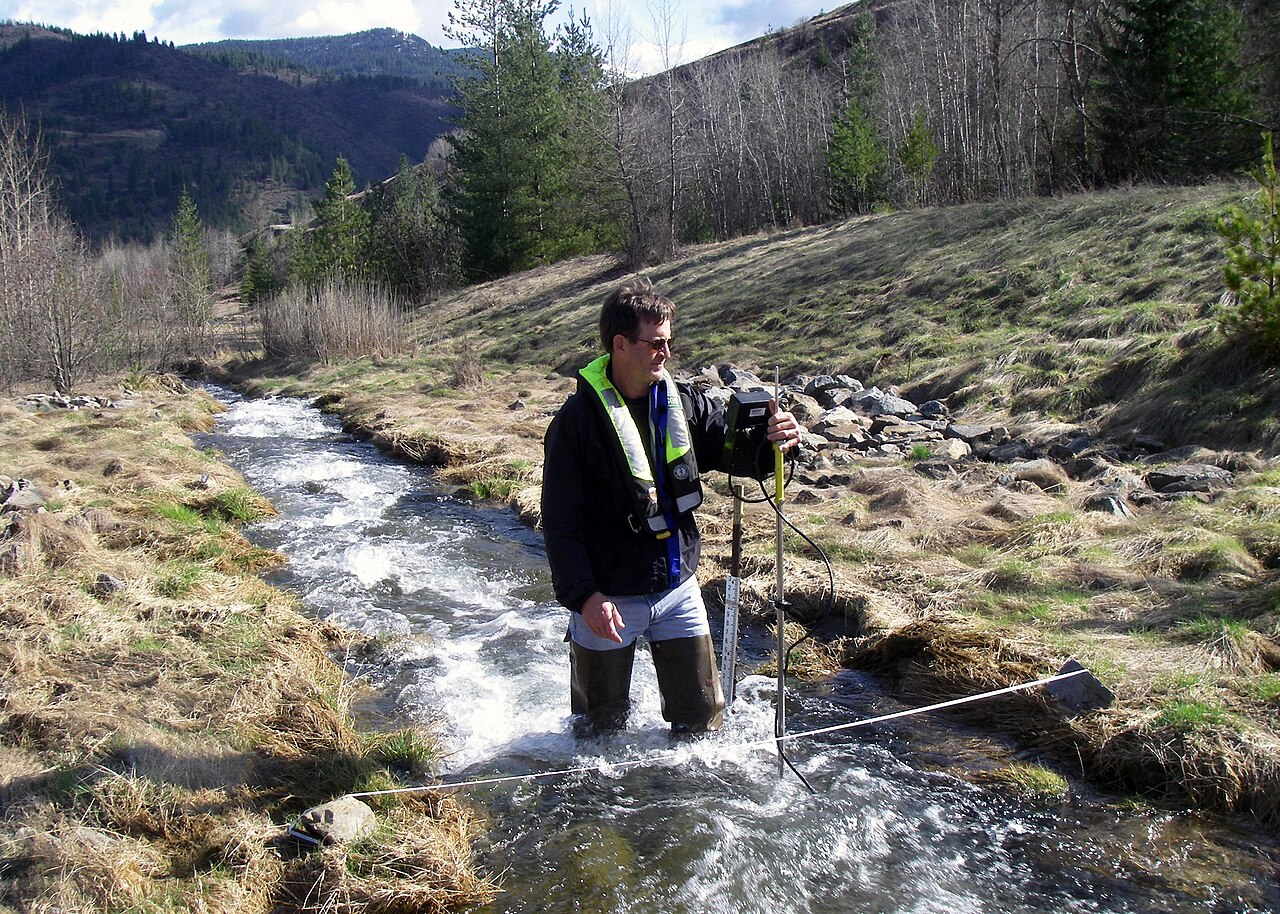
\includegraphics[height=4.6cm]{images/book2/g10-usgs-hydrologist-streamflow.jpg}\hspace{0.3cm}%
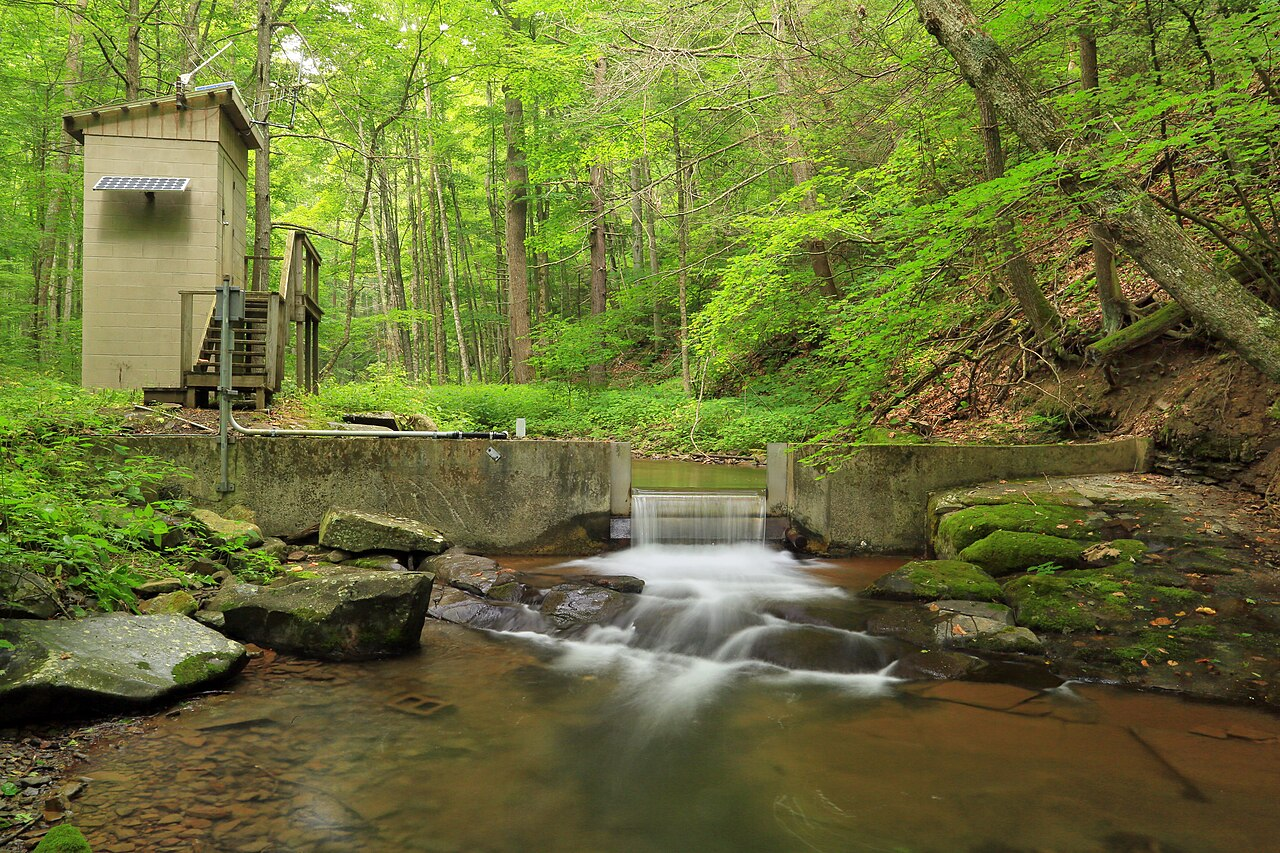
\includegraphics[height=4.6cm]{images/book2/g10-usgs-streamgage.jpg}

{\small Kiri: seorang hidrolog mengukur \omterm{def:g10:drainage-basins:discharge}{debit} sebuah anak sungai pegunungan
dengan metode kecepatan--luas; pita ukur yang dibentangkan melintasi aliran
menandai garis-garis tegak, dan tongkatnya membawa pengukur arus. Kanan:
sebuah stasiun pengukur \omterm{def:g10:drainage-basins:discharge}{debit} di anak sungai di hutan; pondok itu menyimpan
instrumen-instrumen yang merekam tinggi muka air di belakang bendung kecil.
Foto: U.S. Geological Survey (domain publik).}
\end{omfigure}

Pengukuran \omterm{def:g10:drainage-basins:discharge}{debit} memerlukan waktu dan tidak dapat dilakukan terus-menerus.
Sebagai gantinya, stasiun pengukur \omterm{def:g10:drainage-basins:discharge}{debit} merekam tinggi muka air, tanpa
terputus. Beberapa pengukuran \omterm{def:g10:drainage-basins:discharge}{debit} yang dilakukan pada tinggi muka air yang
berbeda memberikan kurva yang menghubungkan tinggi muka air dengan \omterm{def:g10:drainage-basins:discharge}{debit}, dan
stasiun itu mengubah setiap tinggi muka air yang direkamnya menjadi \omterm{def:g10:drainage-basins:discharge}{debit}.

Sungai-sungai besar membawa \omterm{def:g10:drainage-basins:discharge}{debit} yang sangat besar. Dari 1972 sampai 2003
Amazon mengalirkan rata-rata sekitar \qty{206000}{m^3/s} ke Samudra Atlantik,
dengan ketelitian sekitar \qty{6}{\percent}: sekitar \qty{17}{\percent} dari
seluruh air tawar yang dibawa sungai-sungai dunia ke laut. Mississippi
membawa rata-rata \num{593000} kaki kubik per detik, sekitar
\qty{16800}{m^3/s}, ke Teluk Meksiko: Amazon membawa sekitar dua belas kali
lebih banyak.
% ledger: callede:amazon, kammerer:mississippi

\section{Hidrograf}

\begin{definition}[Hidrograf; aliran dasar; waktu tunda]\label{def:g10:drainage-basins:hydrograph}
Yang disebut \emph{hidrograf}\index{hidrograf} adalah grafik \omterm{def:g10:drainage-basins:discharge}{debit} sungai di
satu titik terhadap waktu. Yang disebut \emph{aliran dasar}\index{aliran dasar}
adalah bagian \omterm{def:g10:drainage-basins:discharge}{debit} yang dipasok oleh air tanah, yang membuat sungai tetap
mengalir di antara hujan-hujan. Yang disebut
\emph{waktu tunda}\index{waktu tunda} sebuah banjir adalah waktu di antara
puncak curah hujan di daerah aliran dan puncak \omterm{def:g10:drainage-basins:discharge}{debit}.
\end{definition}

\begin{omfigure}
\begin{tikzpicture}[x=1cm, y=1cm, font=\footnotesize]
  \draw[-{Stealth}] (0,0) -- (10.2,0) node[below left] {waktu};
  \draw[-{Stealth}] (0,0) -- (0,5.9) node[above right] {debit};
  % rain bars hanging from the top
  \draw[black!50] (0,5.4) -- (10,5.4);
  \foreach \x/\h in {1.0/0.15, 1.3/0.35, 1.6/0.55, 1.9/0.4, 2.2/0.2} {
    \fill[omWxRain!70] (\x,5.4) rectangle ++(0.28,-\h);
  }
  \node[anchor=south west] at (2.6,5.4) {curah hujan di daerah aliran};
  % baseflow and hydrograph
  \fill[omSea] (0,0.7) -- (2.0,0.7) .. controls (2.8,0.8) and (3.3,3.3) .. (4.0,3.6)
    .. controls (4.6,3.6) and (5.1,2.1) .. (6.0,1.55) .. controls (7.0,1.0) and (8.0,0.85) .. (10,0.8)
    -- (10,0) -- (0,0) -- cycle;
  \fill[omLithAlluv] (0,0) -- (0,0.7) -- (2.0,0.7) .. controls (3.5,0.68) and (5.5,0.75) .. (6.6,0.95)
    .. controls (8,1.0) and (9,0.85) .. (10,0.8) -- (10,0) -- cycle;
  \draw[omDef, line width=1.2pt] (0,0.7) -- (2.0,0.7) .. controls (2.8,0.8) and (3.3,3.3) .. (4.0,3.6)
    .. controls (4.6,3.6) and (5.1,2.1) .. (6.0,1.55) .. controls (7.0,1.0) and (8.0,0.85) .. (10,0.8);
  \draw[black!60, dashed] (2.0,0.7) .. controls (3.5,0.68) and (5.5,0.75) .. (6.6,0.95);
  % lag time
  \draw[black!60, densely dotted] (1.74,4.85) -- (1.74,4.3);
  \draw[black!60, densely dotted] (3.98,3.65) -- (3.98,4.3);
  \draw[{Stealth}-{Stealth}] (1.74,4.3) -- node[above] {waktu tunda} (3.98,4.3);
  % labels
  \node[anchor=west] at (4.2,3.75) {puncak};
  \node[anchor=east, align=right] at (2.9,2.2) {sisi\\naik};
  \node[anchor=west, align=left] at (5.4,2.3) {sisi turun};
  \node[align=center] at (4.5,1.25) {air larian};
  \node at (8.2,0.4) {aliran dasar};
\end{tikzpicture}

{\small \omterm{def:g10:drainage-basins:hydrograph}{Hidrograf} sebuah banjir (skematis). Setelah hujan, \omterm{def:g10:drainage-basins:discharge}{debit} naik sampai
puncak dan turun kembali dengan lebih lambat; luas di bawah kurva adalah
volume air. \omterm{def:g10:drainage-basins:hydrograph}{Aliran dasar}, yang dipasok oleh air tanah, hanya sedikit berubah;
sisanya adalah air larian yang dikirim hujan dengan cepat ke sungai.}
\end{omfigure}

Air dari sebuah hujan badai mencapai sungai pada waktu yang berbeda-beda. Hujan
yang jatuh di dekat alur tiba dalam beberapa menit atau jam; hujan yang jatuh
jauh di hulu memerlukan waktu yang jauh lebih lama, karena harus mengalir
menuruni lereng dan di sepanjang sungai. Karena itu \omterm{def:g10:drainage-basins:discharge}{debit} naik dengan curam,
pada \emph{sisi naik}, selama air dari lereng-lereng terdekat tiba, mencapai
puncak ketika paling banyak air tiba sekaligus, dan turun lebih lambat, pada
\emph{sisi turun}, ketika air terakhir terkuras dari sudut-sudut terjauh
daerah aliran dan dari tanah. Makin luas daerah alirannya, makin panjang \omterm{def:g10:drainage-basins:hydrograph}{waktu
tundanya}: beberapa jam untuk anak sungai yang kecil, beberapa hari untuk
sungai besar.

Sebagian daerah aliran menghasilkan banjir yang \emph{mendadak}, dengan puncak
yang tinggi dan tiba-tiba serta \omterm{def:g10:drainage-basins:hydrograph}{waktu tunda} yang singkat; daerah aliran
lainnya menghasilkan banjir yang lambat dan landai. Hujan yang sama
menghasilkan banjir yang lebih mendadak bila:
\begin{itemize}
  \item daerah aliran itu kecil dan curam, sehingga air menempuh jalan yang
        pendek dan cepat;
  \item tanah hanya membiarkan sedikit air meresap: batuan telanjang,
        lempung, tanah yang sudah jenuh air, tanah yang membeku, dan terutama
        atap, jalan, dan tempat parkir di kota, yang mengirim hampir seluruh
        hujan langsung ke saluran dan anak sungai;
  \item daerah aliran itu memiliki jaringan anak sungai dan saluran yang
        rapat, yang mengumpulkan air dengan cepat.
\end{itemize}
Hutan, tanah yang dalam dan permeabel, serta dataran banjir yang lebar
melakukan sebaliknya: semuanya menahan air dan melepaskannya perlahan, yang
menurunkan dan menunda puncaknya.

\subsection*{Sebuah banjir sungguhan}

Sungai Potomac mengeringkan daerah aliran seluas \num{11560} mil persegi,
sekitar \qty{29900}{km^2}, di hulu sebuah stasiun pengukur \omterm{def:g10:drainage-basins:discharge}{debit} di dekat
Washington, di Amerika Serikat bagian timur. Pada Januari 1996 stasiun itu
merekam \omterm{def:g10:drainage-basins:hydrograph}{hidrograf} di bawah ini.
% ledger: data:b2-usgs-potomac

\begin{omfigure}
\begin{tikzpicture}
\begin{axis}[omrecord, width=0.86\linewidth, height=6cm, xmin=0, xmax=55, ymin=0, ymax=10000,
  xtick={0,10,20,30,40,50}, xticklabels={5 Jan, 15 Jan, 25 Jan, 4 Feb, 14 Feb, 24 Feb},
  ylabel={debit (\unit{m^3/s})}, xlabel={1996},
  tick label style={font=\small}, label style={font=\small},
  scaled y ticks=false, yticklabel style={/pgf/number format/fixed}]
\addplot[omDef, line width=1.1pt, mark=*, mark size=1.1pt] table[x=day, y=q] {figdata/out/grade-10-flood_frequency-hydrograph.dat};
\node[anchor=west, font=\footnotesize] at (axis cs:17,9231) {\qty{9231}{m^3/s} pada 21 Januari};
\draw[black!60, dashed] (axis cs:5,334) -- (axis cs:13,334);
\node[anchor=south, font=\footnotesize] at (axis cs:9,1000) {sekitar \qty{330}{m^3/s}};
\draw[black!60] (axis cs:9,1000) -- (axis cs:9,390);
\end{axis}
\end{tikzpicture}

{\small \omterm{def:g10:drainage-basins:discharge}{Debit} rata-rata harian Sungai Potomac di dekat Washington dari
5 Januari sampai 29 Februari 1996: banjir naik dari \qty{362}{m^3/s} pada
18 Januari menjadi lebih dari \qty{9000}{m^3/s} tiga hari kemudian, lalu turun
kembali selama minggu-minggu berikutnya, dengan kenaikan kedua yang lebih kecil
pada akhir Januari. Data: U.S. Geological Survey, stasiun 01646500.}
\end{omfigure}
% values computed in figdata/grade-10/flood_frequency.py (hydro_peak_m3s 9231, hydro_before_mean 334)

Pada hari-hari sebelum banjir, sungai itu membawa sekitar \qty{330}{m^3/s},
yaitu \omterm{def:g10:drainage-basins:hydrograph}{aliran dasarnya}. Pada 21 Januari rata-rata hariannya mencapai
\qty{9231}{m^3/s}, hampir tiga puluh kali lebih besar. Bila disebarkan ke
seluruh daerah aliran, air yang melewati stasiun pada hari itu akan membentuk
lapisan setebal
$9231 \times 86400 / (29\,900 \times 10^6) \approx \qty{0.027}{m}$, sekitar
\qty{27}{mm}: hujan lebat, yang dikirim dalam satu hari dari seluruh daerah
aliran sekaligus.
% ledger: data:b2-usgs-potomac (hydro_peak_mm_per_day 26.6 in figdata/grade-10/flood_frequency.py)

\section{Banjir dan periode ulangnya}

Seberapa besar banjir yang harus diperhitungkan sebuah kota? Jawabannya
berasal dari masa lalu: stasiun pengukur \omterm{def:g10:drainage-basins:discharge}{debit} yang telah bekerja selama
puluhan tahun telah merekam \omterm{def:g10:drainage-basins:discharge}{debit} terbesar setiap tahun, yaitu \emph{puncak
tahunan}. Puncak-puncak kecil datang hampir setiap tahun, yang besar jarang.
Makin jarang sebuah banjir, makin besar banjir itu.

\begin{definition}[Periode ulang]\label{def:g10:drainage-basins:return-period}
Yang disebut \emph{periode ulang}\index{periode ulang} $T$ sebuah banjir
adalah selang rata-rata, dalam tahun, di antara tahun-tahun yang puncak
tahunannya menyamai atau melampaui banjir itu. Banjir dengan periode ulang
$T$, yaitu \emph{banjir $T$ tahunan}, memiliki peluang $1/T$ untuk disamai
atau dilampaui dalam satu tahun mana pun.
\end{definition}

Banjir seratus tahunan bukanlah banjir yang datang sekali setiap seratus
tahun, seperti jadwal. Banjir itu adalah banjir yang memiliki satu peluang
dari seratus untuk disamai atau dilampaui setiap tahun, tiap tahun, apa pun
yang terjadi pada tahun sebelumnya. Dua banjir seperti itu dapat datang pada
tahun-tahun yang berurutan; satu abad dapat berlalu tanpa satu pun.

\begin{method}[Periode ulang dari catatan puncak tahunan]\label{met:g10:drainage-basins:return-periods}
\begin{enumerate}
  \item Daftarlah puncak tahunan selama $n$ tahun.
  \item Urutkan dari yang terbesar (peringkat $m = 1$) sampai yang terkecil
        (peringkat $m = n$).
  \item Berikan kepada puncak berperingkat $m$ \omterm{def:g10:drainage-basins:return-period}{periode ulang} $T = (n + 1)/m$.
  \item Gambarlah puncak-puncak itu terhadap $T$ pada skala logaritmik $T$,
        lalu bacalah \omterm{def:g10:drainage-basins:discharge}{debit} untuk \omterm{def:g10:drainage-basins:return-period}{periode ulang} yang diinginkan.
\end{enumerate}
\end{method}

Dengan demikian, yang terbesar dari $n$ puncak mendapat $T = n + 1$ tahun:
dalam catatan \num{95} tahun, \num{96} tahun. Rumus itu mencerminkan apa yang
diperlihatkan catatan: puncak berperingkat $m$ telah disamai atau dilampaui
dalam $m$ dari $n$ tahun, kira-kira sekali setiap $n/m$ tahun. Metode itu
tidak dapat dengan andal menjangkau melampaui panjang catatan: catatan
\num{50} tahun hanya sedikit memberi tahu tentang banjir \num{1000} tahunan.

\begin{omfigure}
\begin{tikzpicture}
\begin{axis}[omrecord, width=0.86\linewidth, height=6.2cm, xmode=log, xmin=0.9, xmax=150,
  ymin=0, ymax=15000, xlabel={periode ulang $T$ (tahun)}, ylabel={puncak tahunan (\unit{m^3/s})},
  xtick={1,2,5,10,20,50,100}, xticklabels={1,2,5,10,20,50,100},
  tick label style={font=\small}, label style={font=\small},
  scaled y ticks=false, yticklabel style={/pgf/number format/fixed}]
\addplot[only marks, mark=*, mark size=1.5pt, omDef] table[x=T, y=peak] {figdata/out/grade-10-flood_frequency-ranked.dat};
\node[anchor=east, font=\footnotesize] at (axis cs:92,13705) {1936};
\node[anchor=east, font=\footnotesize] at (axis cs:46,12658) {1942};
\node[anchor=south, font=\footnotesize] at (axis cs:32,10300) {1972};
\node[anchor=north west, font=\footnotesize, align=left] at (axis cs:1.1,14000) {Sungai Potomac di dekat Washington,\\puncak tahunan 1931--2025 ($n = 95$)};
\end{axis}
\end{tikzpicture}

{\small Ke-\num{95} puncak tahunan Sungai Potomac di dekat Washington,
diurutkan dan digambar terhadap \omterm{def:g10:drainage-basins:return-period}{periode ulangnya} $T = (n+1)/m$. Yang terbesar,
pada Maret 1936, mendapat $T = 96$ tahun. Data: U.S. Geological Survey,
stasiun 01646500.}
\end{omfigure}
% values computed in figdata/grade-10/flood_frequency.py

\begin{dated}{2026}
Dalam catatan Sungai Potomac di dekat Washington, dari 1931 sampai 2025, lima
puncak tahunan terbesar terjadi pada Maret 1936 (\qty{13700}{m^3/s}), Oktober
1942, Juni 1972, April 1937, dan Januari 1996, dua yang terakhir sama besar,
yaitu \qty{9830}{m^3/s}.
% ledger: data:b2-usgs-potomac
\end{dated}

\subsection*{Peluang banjir selama bertahun-tahun}

Rumah atau jembatan berdiri selama puluhan tahun. Yang penting baginya bukanlah
peluang banjir dalam satu tahun, melainkan selama seluruh umurnya.

\begin{proposition}[Sekurang-kurangnya satu banjir dalam $N$ tahun]\label{prop:g10:drainage-basins:chance}
Jika tahun-tahun itu saling bebas, peluang bahwa banjir dengan \omterm{def:g10:drainage-basins:return-period}{periode ulang}
$T$ disamai atau dilampaui sekurang-kurangnya sekali dalam $N$ tahun adalah
\[
P = 1 - \left(1 - \frac{1}{T}\right)^{N}.
\]
\end{proposition}

\begin{proof}
Dalam satu tahun, peluang bahwa banjir itu \emph{tidak} terjadi adalah
$1 - 1/T$. Karena tahun-tahun itu saling bebas, peluang bahwa banjir itu tidak
terjadi dalam satu pun dari $N$ tahun adalah hasil kali $N$ faktor seperti
itu, $(1 - 1/T)^N$. Kejadian ``sekurang-kurangnya sekali'' adalah lawan dari
``tidak pernah'', sehingga peluangnya adalah
$1 - (1 - 1/T)^N$.
\end{proof}

Untuk banjir seratus tahunan selama tiga puluh tahun,
$(0.99)^{30} \approx 0.740$, dan $P \approx 0.26$: satu peluang dari empat. Selama seratus tahun,
$(0.99)^{100}
\approx 0.366$ dan $P \approx 0.63$: banjir seratus tahunan jauh dari pasti
datang dalam seratus tahun.

\begin{omfigure}
\begin{tikzpicture}
\begin{axis}[omrecord, width=0.82\linewidth, height=5.8cm, xmin=0, xmax=100, ymin=0, ymax=1,
  xlabel={banyaknya tahun $N$}, ylabel={peluang sekurang-kurangnya satu banjir},
  ytick={0,0.2,0.4,0.6,0.8,1}, yticklabels={0, 20\,\%, 40\,\%, 60\,\%, 80\,\%, 100\,\%},
  tick label style={font=\small}, label style={font=\small},
  legend pos=south east, legend style={font=\footnotesize}]
\addplot[omThm, line width=1pt] table[x=n, y=p10] {figdata/out/grade-10-flood_frequency-chance.dat};
\addplot[omProp, line width=1pt] table[x=n, y=p50] {figdata/out/grade-10-flood_frequency-chance.dat};
\addplot[omDef, line width=1pt] table[x=n, y=p100] {figdata/out/grade-10-flood_frequency-chance.dat};
\legend{{banjir 10 tahunan}, {banjir 50 tahunan}, {banjir 100 tahunan}}
\draw[black!60, dashed] (axis cs:30,0) -- (axis cs:30,0.2603) -- (axis cs:0,0.2603);
\fill[omDef] (axis cs:30,0.2603) circle (2pt);
\node[anchor=north west, font=\footnotesize] at (axis cs:31,0.22) {26\,\% dalam 30 tahun};
\end{axis}
\end{tikzpicture}

{\small Peluang bahwa banjir dengan \omterm{def:g10:drainage-basins:return-period}{periode ulang} 10, 50, atau 100 tahun
datang sekurang-kurangnya sekali dalam $N$ tahun.}
\end{omfigure}
% values computed in figdata/grade-10/flood_frequency.py (chance_100_30 0.2603)

\section{Bendungan dan tanggul}

Sejak lama manusia membangun bangunan-bangunan yang mengubah cara banjir
lewat. Dua di antaranya mengubahnya dengan cara yang berlawanan.

\emph{Bendungan} menahan sebuah waduk. Ketika banjir tiba, sebagian airnya
disimpan di waduk, yang muka airnya naik, dan dilepaskan sesudahnya, selama
waktu yang lebih panjang. Di hilir, volume air yang sama lewat, tetapi
tersebar: puncaknya lebih rendah dan lebih lambat. Waduk hanya menurunkan
banjir selama masih ada ruang tersisa; begitu penuh, seluruh air yang
memasukinya diteruskan.

\emph{Tanggul} adalah timbunan tanah yang dibangun di sepanjang sungai untuk
menahan banjirnya agar tidak masuk ke dataran banjir. Di antara tanggul-tanggul
itu air tidak dapat menyebar; untuk membawa \omterm{def:g10:drainage-basins:discharge}{debit} yang sama melalui penampang
yang lebih sempit, air harus berdiri lebih tinggi dan mengalir lebih cepat.
Daratan di balik tanggul tetap kering, selama tanggul bertahan dan tidak
terlampaui. Namun dataran banjir tidak lagi menyimpan air selama banjir,
sehingga lebih banyak air, dan lebih cepat, bergerak ke hilir.

\begin{omfigure}
\begin{tikzpicture}[x=0.62cm, y=0.62cm, font=\footnotesize]
  \begin{scope}
    \draw[-{Stealth}] (0,0) -- (9.4,0) node[below left] {waktu};
    \draw[-{Stealth}] (0,0) -- (0,6.0) node[above right] {debit};
    \draw[omDef, line width=1.2pt] (0,0.6) -- (1,0.6) .. controls (1.8,0.7) and (2.2,5.2) .. (2.8,5.2)
      .. controls (3.5,5.2) and (4,1.6) .. (5,1.0) .. controls (6,0.7) and (7.5,0.6) .. (9,0.6);
    \draw[omThm, line width=1.2pt, dashed] (0,0.6) -- (1.3,0.6) .. controls (2.3,0.75) and (3.0,3.3) .. (3.8,3.3)
      .. controls (4.7,3.3) and (5.8,1.5) .. (6.8,1.0) .. controls (7.6,0.75) and (8.3,0.65) .. (9,0.6);
    \node[anchor=west, text=omDef] at (3.0,5.35) {masuk ke waduk};
    \node[anchor=west, text=omThm] at (4.2,3.55) {di hilir bendungan};
    \node[anchor=north] at (4.5,-0.45) {(a) bendungan: puncak lebih rendah dan lebih lambat};
  \end{scope}
  \begin{scope}[xshift=7.2cm]
    \fill[omLithAlluv] (0,0) -- (10,0) -- (10,1.8) -- (0,1.8) -- cycle;
    \fill[white] (3.5,1.8) -- (3.9,0.4) -- (6.1,0.4) -- (6.5,1.8) -- cycle;
    \fill[omSea] (0.4,2.3) -- (3.25,2.3) -- (3.5,1.8) -- (3.9,0.4) -- (6.1,0.4) -- (6.5,1.8) -- (6.75,2.3) -- (9.6,2.3) -- (9.6,1.8) -- (0.4,1.8) -- cycle;
    \draw[line width=0.8pt, brown!60!black] (0,1.8) -- (3.5,1.8) -- (3.9,0.4) -- (6.1,0.4) -- (6.5,1.8) -- (10,1.8);
    \draw[omDef!70!black] (0.4,2.3) -- (9.6,2.3);
    \node[anchor=south, text=omDef!70!black, align=center] at (1.5,2.35) {tanpa\\tanggul};
    % levees
    \fill[brown!45] (2.6,1.8) -- (3.0,3.9) -- (3.3,3.9) -- (3.5,1.8) -- cycle;
    \fill[brown!45] (6.5,1.8) -- (6.7,3.9) -- (7.0,3.9) -- (7.4,1.8) -- cycle;
    \fill[omSea!70!omDef] (3.5,1.8) -- (3.9,0.4) -- (6.1,0.4) -- (6.5,1.8) -- (6.65,3.4) -- (3.35,3.4) -- cycle;
    \draw[omThm, line width=0.8pt, dashed] (3.35,3.4) -- (6.65,3.4);
    \node[anchor=south, text=omThm] at (5,3.95) {dengan tanggul};
    \draw[omThm] (5,3.95) -- (5,3.45);
    \node[anchor=north] at (5,-0.45) {(b) tanggul: banjir berdiri lebih tinggi};
  \end{scope}
\end{tikzpicture}

{\small Skematis. (a) Waduk menyimpan sebagian banjir dan melepaskannya
kemudian: di hilir bendungan puncaknya lebih rendah dan datang lebih lambat.
(b) Tanpa tanggul, banjir menyebar tipis di atas dataran banjir; di antara
tanggul, \omterm{def:g10:drainage-basins:discharge}{debit} yang sama harus melewati penampang yang sempit dan berdiri jauh
lebih tinggi.}
\end{omfigure}

\section{Latihan}

\begin{exercise}[$\star$]\label{exo:g10:drainage-basins:1}
Definisikan \omterm{def:g10:drainage-basins:drainage-basin}{daerah aliran sungai} dan \omterm{def:g10:drainage-basins:drainage-basin}{garis pemisah air}. Mengapa dua tetes
hujan yang jatuh berjarak satu meter dapat berakhir di dua laut yang berbeda?
\end{exercise}

\begin{exercise}[$\star$]\label{exo:g10:drainage-basins:2}
Definisikan \omterm{def:g10:drainage-basins:discharge}{debit} sungai dan sebutkan satuannya. Berapa liter air yang
melewati suatu titik di sungai yang membawa \qty{1}{m^3/s} dalam sehari?
\end{exercise}

\begin{exercise}[$\star$]\label{exo:g10:drainage-basins:3}
Pada \omterm{def:g10:drainage-basins:hydrograph}{hidrograf} Sungai Potomac bulan Januari 1996, bacalah \omterm{def:g10:drainage-basins:hydrograph}{aliran dasar}
sebelum banjir, \omterm{def:g10:drainage-basins:discharge}{debit} puncak beserta tanggalnya, dan banyaknya hari yang
diperlukan oleh kenaikan itu.
\end{exercise}

\begin{exercise}[$\star$]\label{exo:g10:drainage-basins:4}
Berapa peluang bahwa banjir \num{50} tahunan disamai atau dilampaui tahun
depan? Banjir \num{50} tahunan datang tahun lalu: apakah peluangnya lebih
kecil tahun ini?
\end{exercise}

\begin{exercise}[$\star$]\label{exo:g10:drainage-basins:5}
Mississippi membawa rata-rata \num{593000} kaki kubik air per detik ke laut
(\num{1}~kaki = \qty{0.3048}{m}). Ubahlah \omterm{def:g10:drainage-basins:discharge}{debit} ini ke \unit{m^3/s}, lalu
bandingkan dengan \qty{206000}{m^3/s} milik Amazon.
\end{exercise}

\begin{exercise}[$\star\star$]\label{exo:g10:drainage-basins:6}
Seorang hidrolog mengukur \omterm{def:g10:drainage-basins:discharge}{debit} sebuah anak sungai dengan empat garis tegak
berjarak \qty{1.5}{m}. Kedalamannya \num{0.3}, \num{0.6}, \num{0.7}, dan
\qty{0.4}{m}; kecepatan rata-ratanya \num{0.2}, \num{0.5}, \num{0.6}, dan
\qty{0.3}{m/s}. Hitung penampang, \omterm{def:g10:drainage-basins:discharge}{debit}, dan kecepatan rata-ratanya.
\end{exercise}

\begin{exercise}[$\star\star$]\label{exo:g10:drainage-basins:7}
Sebuah hujan badai menurunkan hujan \qty{20}{mm} di atas seluruh daerah aliran
Sungai Varden pada peta, \qty{66}{km^2}. Berapa volume air itu? Jika seluruhnya
mencapai titik keluaran dalam dua hari, berapa \omterm{def:g10:drainage-basins:discharge}{debit} tambahan rata-ratanya?
\end{exercise}

\begin{exercise}[$\star\star$]\label{exo:g10:drainage-basins:8}
Puncak tahunan sebuah sungai kecil selama sembilan tahun adalah, dalam
\unit{m^3/s}: \num{42}, \num{65}, \num{38}, \num{120}, \num{51}, \num{47},
\num{88}, \num{35}, \num{59}. Urutkan puncak-puncak itu dan sebutkan \omterm{def:g10:drainage-basins:return-period}{periode
ulang} tiga yang terbesar. Berapa \omterm{def:g10:drainage-basins:return-period}{periode ulang} puncak mediannya?
\end{exercise}

\begin{exercise}[$\star\star$]\label{exo:g10:drainage-basins:9}
Hujan badai yang sama jatuh di dua daerah aliran yang luasnya sama: satu
curam dan tertutup oleh kota, yang lain landai dan berhutan. Sketsalah kedua
\omterm{def:g10:drainage-basins:hydrograph}{hidrograf} itu pada sumbu yang sama dan jelaskan perbedaannya.
\end{exercise}

\begin{exercise}[$\star\star$]\label{exo:g10:drainage-basins:10}
Pada puncak 21 Januari 1996, Sungai Potomac membawa \qty{9231}{m^3/s} dari
daerah aliran seluas \qty{29900}{km^2}. Berapa tebal air, bila disebarkan ke
seluruh daerah aliran, yang diwakili oleh satu hari \omterm{def:g10:drainage-basins:discharge}{debit} ini? Bandingkan
dengan \omterm{def:g10:drainage-basins:hydrograph}{aliran dasar} \qty{330}{m^3/s}.
\end{exercise}

\begin{exercise}[$\star\star$]\label{exo:g10:drainage-basins:11}
Berapa peluang bahwa banjir \num{10} tahunan datang sekurang-kurangnya sekali
dalam \num{10} tahun? Bahwa banjir itu sama sekali tidak datang dalam sepuluh
tahun ini?
\end{exercise}

\begin{exercise}[$\star\star\star$]\label{exo:g10:drainage-basins:12}
\omterm{def:g10:drainage-basins:discharge}{Debit} yang memasuki sebuah waduk saat banjir naik secara teratur dari
\qty{0}{m^3/s} menjadi \qty{1200}{m^3/s} dalam satu hari, lalu turun secara
teratur kembali menjadi \qty{0}{m^3/s} dalam dua hari (\omterm{def:g10:drainage-basins:hydrograph}{aliran dasar}
diabaikan). Berapa volume yang dibawa banjir itu? Bendungan itu meloloskan
paling banyak \qty{800}{m^3/s}, dan waduknya dapat menyimpan \num{60} juta
\unit{m^3}. Dapatkah waduk itu menahan semua yang di atas \qty{800}{m^3/s}?
\end{exercise}

\begin{exercise}[$\star\star\star$]\label{exo:g10:drainage-basins:13}
Sebuah sungai selebar \qty{100}{m} penuh sampai ke tepiannya pada
\qty{800}{m^3/s}, dengan kecepatan \qty{2}{m/s}. Banjir \qty{1200}{m^3/s} tiba.
\begin{enumerate}
  \item Tanpa tanggul, tambahan \qty{400}{m^3/s} menyebar di atas dataran
        banjir selebar \qty{900}{m}, tempat air mengalir dengan kecepatan
        \qty{0.5}{m/s}. Berapa dalam air di dataran banjir?
  \item Dengan tanggul, seluruh banjir lewat di antara tanggul-tanggul itu,
        dengan kecepatan \qty{2}{m/s}. Berapa dalam sungai itu, dan setinggi
        apa sungai itu berdiri di atas tepiannya?
\end{enumerate}
\end{exercise}

\begin{exercise}[$\star\star\star$]\label{exo:g10:drainage-basins:14}
\omterm{def:g10:drainage-basins:return-period}{Periode ulang} $T$ berapakah yang memberi sebuah banjir peluang satu dari dua
untuk datang sekurang-kurangnya sekali dalam \num{30} tahun?
\end{exercise}

\begin{exercise}[$\star\star\star$]\label{exo:g10:drainage-basins:15}
Sebuah peta kecil dipotong menjadi persegi-persegi bersisi \qty{100}{m};
ketinggiannya dalam meter diberikan di bawah (utara di atas). Air
meninggalkan setiap persegi menuju tetangga terendah dari keempat tetangganya
(utara, selatan, timur, barat) jika tetangga itu lebih rendah; persegi pada
\qty{34}{m} (sudut barat laut) dan \qty{30}{m} (sudut tenggara) adalah titik
keluaran dua anak sungai.
\begin{center}
\begin{tabular}{|c|c|c|c|}
\hline
34 & 38 & 46 & 50 \\ \hline
37 & 42 & 48 & 47 \\ \hline
45 & 49 & 44 & 39 \\ \hline
51 & 46 & 37 & 30 \\ \hline
\end{tabular}
\end{center}
Gambarlah arah aliran setiap persegi, temukan daerah aliran setiap titik
keluaran beserta luasnya, dan gambarlah \omterm{def:g10:drainage-basins:drainage-basin}{garis pemisah airnya}.
\end{exercise}

\section{Soal: Banjir Seratus Tahunan}

\begin{problem}[{Soal akhir pekan --- seberapa sering sungai masuk ke kota?}]
\label{pb:g10:drainage-basins:1}
% ledger: data:b2-usgs-potomac (values computed in figdata/grade-10/flood_frequency.py)
Bayangkan sebuah kota di tepi Sungai Potomac, sedikit di hulu Washington, di
dekat stasiun pengukur \omterm{def:g10:drainage-basins:discharge}{debit} yang telah merekam \omterm{def:g10:drainage-basins:discharge}{debit} terbesar sungai itu
setiap tahun sejak 1931. Puncak-puncak tahunannya digambar di bawah ini, dan
\omterm{def:g10:drainage-basins:hydrograph}{hidrograf} Januari 1996 diberikan dalam bab ini.

\begin{center}
\begin{tikzpicture}
\begin{axis}[omrecord, width=0.9\linewidth, height=5.4cm, ybar, bar width=1.6pt, xmin=1929, xmax=2027,
  ymin=0, ymax=15000, ylabel={puncak tahunan (\unit{m^3/s})}, xlabel={tahun},
  xtick={1930,1950,1970,1990,2010}, xticklabel style={/pgf/number format/1000 sep={}},
  tick label style={font=\small}, label style={font=\small},
  scaled y ticks=false, yticklabel style={/pgf/number format/fixed}]
\addplot[fill=omDef!70, draw=none] table[x=year, y=peak] {figdata/out/grade-10-flood_frequency-record.dat};
\draw[omThm, dashed] (axis cs:1929,9500) -- (axis cs:2027,9500);
\node[anchor=south east, font=\footnotesize, text=omThm] at (axis cs:2026,9500) {\qty{9500}{m^3/s}};
\end{axis}
\end{tikzpicture}

{\small \omterm{def:g10:drainage-basins:discharge}{Debit} puncak tahunan Sungai Potomac di dekat Washington, tahun air
1931--2025 (tahun air berlangsung dari Oktober sampai September: banjir
Oktober 1942 dihitung pada 1943). Data: U.S. Geological Survey, stasiun
01646500.}
\end{center}

\medskip
\noindent\textbf{Bagian I --- Daerah aliran dan debit.}
\begin{enumerate}
  \item Daerah aliran stasiun itu meliputi \num{11560} mil persegi
        (\num{1}~mil = \qty{1.609}{km}). Ubahlah luas ini ke
        \unit{km^2}.
  \item Garis apa pada peta yang membatasi wilayah ini?
  \item Puncak terbesar, pada 19 Maret 1936, adalah \num{484000} kaki kubik
        per detik. Ubahlah ke \unit{m^3/s} (\num{1}~kaki =
        \qty{0.3048}{m}).
  \item Puncak tahunan median adalah \qty{3341}{m^3/s}. Berapa kali lebih
        besar banjir tahun 1936 dibandingkan dengan median itu?
  \item Misalkan pada puncak tahun 1936 sungai itu rata-rata selebar
        \qty{400}{m} dan sedalam \qty{8}{m} di stasiun. Berapa kecepatan
        rata-ratanya?
\end{enumerate}

\medskip
\noindent\textbf{Bagian II --- Membaca banjir tahun 1996.}
\begin{enumerate}[resume]
  \item Pada \omterm{def:g10:drainage-basins:hydrograph}{hidrograf} Januari 1996, berapa \omterm{def:g10:drainage-basins:hydrograph}{aliran dasar} pada hari-hari
        sebelum banjir?
  \item Berapa \omterm{def:g10:drainage-basins:discharge}{debit} harian puncaknya, dan pada hari apa?
  \item Berapa hari yang diperlukan oleh kenaikan itu, dari
        \qty{362}{m^3/s} pada 18 Januari sampai puncaknya?
  \item Berapa tebal air di seluruh daerah aliran yang dibawa melewati
        stasiun pada hari puncak?
  \item Kenaikan kedua yang lebih kecil mencapai puncak pada 29 Januari. Apa
        yang diberitahukannya tentang air yang mencapai daerah aliran?
  \item \omterm{def:g10:drainage-basins:discharge}{Debit} kembali mendekati \qty{410}{m^3/s} pada 7 Februari. Berapa lama
        setelah puncak itu? Mengapa sisi turun berlangsung lebih lama daripada
        sisi naik?
\end{enumerate}

\medskip
\noindent\textbf{Bagian III --- Mengurutkan banjir.}
\begin{enumerate}[resume]
  \item Catatan itu memuat $n = 95$ puncak tahunan. \omterm{def:g10:drainage-basins:return-period}{Periode ulang} berapa yang
        diberikan metode itu kepada yang terbesar?
  \item Puncak Oktober 1942 (\qty{12658}{m^3/s}) berperingkat kedua. Berapa
        \omterm{def:g10:drainage-basins:return-period}{periode ulangnya}?
  \item Puncak Juni 1972 (\qty{10166}{m^3/s}) berperingkat ketiga. Berapa
        \omterm{def:g10:drainage-basins:return-period}{periode ulangnya}?
  \item Banjir April 1937 dan Januari 1996 sama besar (\qty{9826}{m^3/s}).
        Bila diberi peringkat 4 dan 5, \omterm{def:g10:drainage-basins:return-period}{periode ulang} berapa yang diperolehnya?
        Apakah nilai yang sama itu banyak berpengaruh di sini?
  \item Pada diagram batang, hitunglah tahun-tahun yang puncaknya melampaui
        \qty{9500}{m^3/s}. Perkirakan peluang puncak seperti itu dalam satu
        tahun mana pun, dan \omterm{def:g10:drainage-basins:return-period}{periode ulangnya}.
\end{enumerate}

\medskip
\noindent\textbf{Bagian IV --- Peluang banjir.}
\begin{enumerate}[resume]
  \item Berapa peluang bahwa banjir \num{100} tahunan disamai atau dilampaui
        dalam satu tahun tertentu?
  \item Berapa peluang bahwa banjir itu tidak disamai atau dilampaui, pada
        tahun itu?
  \item Berapa peluang bahwa banjir itu tidak datang dalam \num{30} tahun,
        yaitu lamanya sebuah keluarga mungkin tinggal di rumah di tepi sungai?
  \item Berapa peluang sekurang-kurangnya satu banjir \num{100} tahunan dalam
        \num{30} tahun?
\end{enumerate}
\end{problem}
